\section{Swing Leg Control}\label{sec:neuro_swing_reflexes} 

During swing, the reflexes shape the natural double pendulum dynamics of the leg
in order to achieve sufficient knee flexion, prevent toe scuffing, reach a
target landing leg angle, and then extend the leg towards the ground. We here
review an idealized control model, proposed in \citet{desai2012robust}, which
proposes reflexes that directly apply torques to the hip and knee joints.

The idealized swing control comprises two layers. In the first layer, a leg
placement policy,
\begin{align}
    \alpha_{\tn{tgt}} = \alpha_{0} + c_\tn{d} d + c_\tn{v} v,
    \label{eq:simbicon}
\end{align}
prescribes leg angle for the leg to reach by the end of swing. We measure the
leg angle between the hip-ankle line and horizontal as shown in
\cref{fig:swing_leg_polar}. In \cref{eq:simbicon}, $\alpha_{\tn{tgt}}$ is the
target leg angle, $\alpha_{0}$ is the default leg angle, $d$ is the horizontal
distance between the stance leg ankle and the model's center of mass, $v$ is the
velocity of the center of mass, and $c_\tn{d}$ and $c_\tn{v}$ are constant gain
parameters. This policy is taken from~\citet{yin2007simbicon} and represents an
empirical generalization of the leg placement strategies that recover the linear
inverted pendulum model of human walking from
disturbances~\citep{kajita20013d,pratt2006capture}. 
\begin{marginfigure}[-2in]
    \centering
    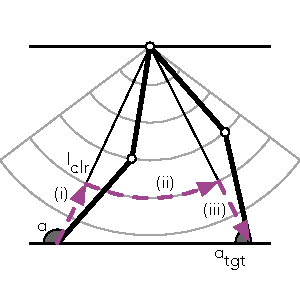
\includegraphics[width=\linewidth]{swing_leg_polar}
    \caption[The idealized swing leg control guides the leg towards a desired
    landing leg angle $\alpha_\tn{tgt}$ through three phases]{The idealized
    swing leg control guides the leg towards a desired landing leg angle
    $\alpha_\tn{tgt}$ through three phases: (i) Flex the knee until it achieves
    a clearance leg length $l_\tn{clr}$. (ii) Hold the leg length via knee
    damping. (iii) Stop and Extend the leg towards the ground when the leg
    reaches $\alpha_\tn{tgt}$. Figure reproduced from
    \citet{desai2012robust}.}\label{fig:swing_leg_polar}
\end{marginfigure}

The target angle generated by this policy forms a central input to the second
layer comprised of hip and knee controls. The portion of this control that
governs the knee action uses a finite state machine to switch between three
phases. The first phase allows the knee to passively flex in response to hip
moments generated at the onset of swing. If the passive knee flexion is
insufficient (the foot swings forward with a tendency to scuff the ground), the
control produces active flexion torque of the knee in proportion to the rate
$\dot{\alpha}$ of forward leg motion,
\begin{align}
    \tau_\tn{k}^\tn{i} = \begin{cases}
                 0,                     & \dot{\alpha} > 0 \\
                -k^\tn{i} \dot{\alpha}, & \dot{\alpha} \le 0 
                \end{cases},
    \label{eq:flexphase}
\end{align}
where $k^\tn{i}$ is the flexion gain and the leg angle $\alpha$ is defined as
the angle between the horizontal and the hip-ankle line.  

The second phase activates when the leg length, defined as the distance between
the hip and ankle, contracts below a threshold. In this phase, the knee torque
is given by
\begin{align}
    \tau_\tn{k}^\tn{ii} = \begin{cases}
          -k_1^\tn{ii} \dot \phi_\tn{k}, & \dot \phi_\tn{k} \ge 0 \\
          -k_2^\tn{ii} \dot \phi_\tn{k}(\alpha - \alpha_\tn{tgt})
            (\dot{\alpha} - \dot \phi_\tn{k}), 
          & \dot\phi_\tn{k} < 0 \ \& \ \dot \phi_\tn{k} < \dot \alpha\\
          0, & \mathrm{otherwise}
      \end{cases},
    \label{eq:holdphase}
\end{align}
where $k_1^\tn{ii}$ and $k_2^\tn{ii}$ are damping coefficients. The first case
dampens knee flexion, while the second case dampens knee extension, but allows
progressively more extension as the leg angle approaches its target. The
modulation term $(\dot \alpha - \dot \phi_\tn{k})$ prevents premature landing of
the leg by damping the knee if it extends faster than the overall leg angle.

The third phase engages when the leg angle gets within a threshold of the
target leg angle. The control then applies torque to stop and extend the knee,  
\begin{align}
    \tau_k^\tn{iii} = 
    \begin{cases}
         k^\tn{iii}(\alpha_{\tn{thr}} - \alpha)
            \left(1 - \frac{\dot\alpha}{\dot\alpha_\tn{max}} \right), 
                & \alpha < \alpha_\tn{thr} \ \& \ \dot \alpha < \dot \alpha_\tn{max} \\
        0, & \tn{otherwise}
    \end{cases},
    \label{eq:stop}
\end{align}
where $\dot{\alpha}_{\mathrm{max}}$ is the maximum leg retraction velocity for
which the stopping knee torque is applied. When this torque brings the leg
velocity to zero, a knee extension torque is added,
\begin{align}
    \tau_\tn{k}^\tn{iii'} = \tau_\tn{k}^\tn{iii} - k^\tn{ext} (l_0 - l),
    \label{eq:extend}
\end{align}
where $l_0$ is the rest leg length, $l$ is the current leg length, and
$k^\tn{ext}$ is a proportional gain. 

The swing leg control also specifies a hip torque in the form of a proportional
derivative control on the leg angle, 
\begin{align}
    \tau_\tn{h}^\alpha = k_\tn{p} (\alpha - \alpha_\tn{tgt}) + k_\tn{d} \dot\alpha.
    \label{eq:hipfeedback}
\end{align}
This hip torque is supplemented by a feed forward term 
\begin{align}
    \tau_\tn{h} = \tau_\tn{h}^\alpha - 2 \tau_\tn{k}^\tn{iii}
    \label{eq:hipfeedforward}
\end{align} 
that neutralizes the coupling dynamics between the knee and hip during the
knee's stop and extend phase (Eq.~\ref{eq:stop}).
